\documentclass[11pt]{article}
\usepackage[margin=1in]{geometry}
\usepackage{amsmath,amsthm,amssymb}
\usepackage{float}
\usepackage{hyperref}
\usepackage{booktabs}
\usepackage{placeins}
\usepackage{graphicx}
\usepackage[
backend=biber,
style=bwl-FU,
sorting=ynt
]{biblatex}
\addbibresource{../main.bib}

\DeclareMathOperator*{\argmax}{arg\,max}
\DeclareMathOperator*{\argmin}{arg\,min}

\title{Model Updates and Results}
\author{José I. Velarde Morales}

\begin{document}
\maketitle
\section{Modifications to Model}
    \subsection{Simplified Ideal Model}

    The first model we proposed aimed to minimize the probability that a farmer's net loss would exceed an exogenously given threshold. This was subject to a maximum premium constraint and a constraint specifying a piecewise linear structure for the payout function. Index insurance contracts are generally defined by three values: a trigger value, $t$, an exit value $e$, and a maximum payout $K$. Given these values and a specific value of $\theta$, the payout would be: $I(\theta) = K \cdot \min \{ \max \{0,\frac{\theta - t}{e-t} \},1 \}$. Note that this can also be expressed as: $I(\theta) = \min \left \{(a\theta +b)^+,K \right \}$. We opt for the second representation of the class of functions because it is more straightforward to derive a convex approximation for it. In the model below, $\ell$ is the farmer's loss, $\pi$ is the premium he pays, $I(\theta)$ is the insurance payout, $c_k$ is the cost of capital, and $\bar{\ell}$ is the loss threshold we don't want the farmer to exceed. In other words, we want the farmer to have net losses lower than $\bar{\ell}$ with high probability. The premium contains two terms, the first is for the expected payout of the contract, and the second is for the costs of holding the capital necessary to insure the contract. $K^P$ is the amount of capital needed by the insurer to be able to uphold their side of the contract with high probability. $\epsilon$ is determined by regulations on the capital requirements for insurers. The EU, for example, requires that insurance companies have enough capital on hand to be solvent in the case of payouts exceeding the $99^{th}$ percentile of the distribution, this would correspond to $\epsilon=0.01$. For exposition, we first show the optimization model for insuring a single zone, and we then show the model for insuring multiple zones.

    \paragraph*{Single Zone}

    \begin{align}
        \min_{a,b,\pi} P(\ell + \pi &-I(\theta) \geq \bar{\ell})\\
        \text{s.t.   } I(\theta) &= \min \{ (a\theta - b)^+,K \}\\
        \pi &= E[I(\theta)] + c_k K^P\\
        \pi &\leq \bar{\pi}\\
        K^P &= CVaR_{1-\epsilon}\left ( I(\theta) \right ) - \pi
    \end{align}

    \paragraph*{Multiple Zone}
    In the multiple zone case, we minimize the maximum probability across zones that a farmer's wealth will drop below a certain threshold. We minimize the maximum probability across zones to avoid solutions where one zone gets a much worse contract. In the model below, $\rho_z$ is a measure of the relative riskiness of zone $z$, it is meant to capture what share of the cost of capital is due to zone $z$. Intuitively, if a zone is less risky, then it takes less capital to insure it, and that should be reflected in the premium they pay. 

    \begin{align}
        \min_{t,a,b,e,\pi} \max_z P(\ell_z &- \pi_z +I_z(\theta_z) \geq \bar{\ell})\\
        \text{s.t.   } I_z(\theta_z) &= \min \{ (a_z\theta_z + b_z)^+,K_z \}, \forall z\\
        K^P &= CVaR_{1-\epsilon}\left (\sum_z I_z(\theta_z) \right ) - \sum_z \pi_z\\
        \pi_z &= E[I_z(\theta_z)]+c_k K^P \rho_z, \forall z \\
        \pi_z &\leq \bar{\pi}, \forall z
    \end{align}

    \subsection{Old Convex Approximation}
    Since probabilitic constraints are generally non-convex, we also considered trying to minimize the conditional value at risk (CVaR) of the farmer's net loss instead. I think this is a good objective for our context because it minimizes the expected value of the loss in the worse case scenarios. It also has the advantage of having been well studied in the literature, and there are tractable reformulations for having $CV@R$ in the objective and constraints for general loss distributions. This model minimizes the $CV@R$ of the farmer's net loss subject to a constraint on the premium. The premium constraints are expressed as a fraction of the full insured amount. So, if $\bar{\pi}$ is the maximum premium share and $K$ is the full insured amount, then the constraint on the premium would be: $\pi \leq K \bar{\pi}$.

    \subsubsection*{Single Zone Model}
    \paragraph*{Model Parameters}
    \begin{itemize}
        \item $\epsilon$: This defines the CV@R objective. $\epsilon = 0.1$ means that our objective is on the expected value of the loss given that it is above the $90^{th}$ percentile. 
        \item $\epsilon_P$: This is the epsilon corresponding to the $CV@R$ of the payouts. This is used to determine the required capital for the portfolio and is usually set by regulators.
        \item $\bar{\pi}$: This is the maximum value of the premium. 
        \item $K$: maximum insured amount
    \end{itemize}

    \paragraph*{Model}
    \begin{align}
        \min_{a,b\geq 0} &\ CV@R_{1-\epsilon}\left(\ell  - \min \left \{(a\theta + b), K \right \} \right)\\
        \text{s.t.   } &\   a \mathbb{E} \left[\theta \right] + b +c_k K^P \leq K\bar{\pi}\\
        & K^P = CV@R_{1-\epsilon_P} \left( a\theta +b \right) - a \mathbb{E} \left[\theta \right] + b\\
        & a\theta + b \geq 0 
    \end{align}

    % We reformulated the problem in the following way. In the model below, $p_k$ is the probability of event $k$, and $k$ indexes the possible realizations of $\theta, \ell$.

    % \begin{align}
    %     \min_{a,b,\gamma,t} &\quad t + \frac{1}{\epsilon}\sum_k p_k \gamma_k\\
    %     \text{s.t.   } \gamma_k &\geq \ell^k - \min\left\{(a\hat{\ell}(\theta^k) + b), K\right\} - t, \forall k\\
    %     \gamma_k &\geq 0, \forall k \\
    %     0 &\leq a\hat{\ell}(\theta^k) + b, \forall k\\
    %     K\bar{\pi} &\geq a\mathbb{E}[\hat{l}(\theta)] + b
    % \end{align}

    \subsubsection*{Multiple Zone Model}
    \paragraph*{Model Parameters}
        \begin{itemize}
            \item $\epsilon$: This defines the CV@R objective. $\epsilon = 0.1$ means that our objective is on the expected value of the loss given that it is above the $90^{th}$ percentile. 
            \item $\bar{\pi}, \underline{\pi}$: These are the maximum and minimum values for the premium respectively. 
            \item $\rho_z$: This is a measure of the relative riskiness of zone $z$. 
            \item $\epsilon_P$: This is the epsilon corresponding to the $CV@R$ of the entire portfolio. This is used to determine the required capital for the portfolio. Values I've seen used are $\epsilon_P=0.01$ and $\epsilon_P=0.05$. 
            \item $Z$: number of insured zones.
            \item $c_k$: cost of capital
            \item $K_z$: maximum insured amount of zone $z$.  
        \end{itemize}

        \paragraph*{Model}
        
        \begin{align}
            \min_{a,b,K^P} \max_z &\quad CV@R_{1-\epsilon}(\ell_z - \min\left\{(a_z\hat{\ell_z}(\theta_z) + b_z), K_z\right\})\\
            \text{s.t.   } K\bar{\pi} &\geq a_z \mathbb{E}[\hat{\ell_z}(\theta^k_z)] + b_z + c_k\rho_z K^P,  \forall k, \forall z\\
            0 &\leq a_z\hat{\ell_z}(\theta^k_z) + b_z, \forall k, \forall z \\
            K^P + Z\underline{\pi} &\geq CV@R_{1-\epsilon_P}\left( \sum_z a_z \hat{\ell_z}(\theta_z) + b_z \right)
        \end{align}
        
        % The reformulation is: 
        
        % \begin{align}
        %     \min_{a,b,\gamma,t,m,K^P} \quad & m\\
        %     \text{s.t.} \quad t_z &+ \frac{1}{\epsilon} \sum_k p_k \gamma_z^k \leq m, \forall z\\
        %     \gamma_z^k &\geq \ell^k - \min\left\{(a_z\hat{\ell_z}(\theta_z^k) + b_z), K_z\right\} -t_z, \forall k, \forall z \\
        %     \gamma_z^k &\geq 0, \forall k, \forall z\\
        %     t_p &+ \frac{1}{\epsilon_p} \sum_k p_k \gamma_P^k \leq K^P+Z\underline{\pi}\\
        %     \gamma_P^k &\geq \sum_z a_z \hat{\ell_z}(\theta^k_z) + b_z -t_p, \forall k \\
        %     \gamma_P^k &\geq 0, \forall k\\
        %     K_z\bar{\pi} &\geq a_z \mathbb{E}[\hat{\ell_z}(\theta_z)] + b_z + c_k \beta_z K^P, \forall z \\
        %     0 &\leq a_z \hat{\ell_z}(\theta_z^k) + b_z, \forall k, \forall z
        % \end{align}

    \subsection{New Convex Approximation}
    The original multiple zone model led to unsatisfactory results. One of the problems was that the model did not allow $a\hat{\ell}(\theta)+b$ to be negative. On the one hand, this makes sense because it would mean negative payouts. On the other hand, however, it forced the model to start paying out whenever the predicted loss was non-negative. This meant the model was forced to grant payouts even in cases where the predicted loss was small, this in turn affected the size of the payouts it could give in cases of large losses. Intuitively, we want to save our budget for larger losses, and this functional form was forcing it to spend some of its budget on small losses. We ideally want to optimize over functions of the form: $f(x) = \min \left \{\max \left \{0,a\theta + b \right \}, K \right \}$. To approximate the program over the class of functions we are interested in, we modified the program in the following way. We also changed the premium constraint into an overall budget constraint, to make comparisons with the status quo more straightforward: 
    
    % One of the problems was that the model excluded functions of the form: $f(x) = \max \left \{0,a\theta + b\right \}$, which is the function space we ideally want to optimize over. We ideally want to optimize over functions of the form: $f(x) = \min \left \{\max \left \{0,a\theta + b \right \}, K \right \}$. We want to optimize over this function space because these types of functions are what is traditionally used in index insurance contracts. The reason they are popular is that they start paying out once the loss is deeemed big enough. The problem with the original model is that it was constrained to start paying out whenever the predicted loss was non-negative. This meant the model was forced to grant payouts even in cases where the predicted loss was small, this in turn affected the size of the payouts it could give in cases of large losses. To approximate the program over the class of functions we are interested in, we modified the program in the following way. We also changed the premium constraint into an overall budget constraint, to make comparisons with the status quo more straightforward: 

    \subsubsection*{Single Zone Model}
    \paragraph*{Model Parameters}
    \begin{itemize}
        \item $\epsilon$: This defines the CV@R objective. $\epsilon = 0.1$ means that our objective is on the expected value of the loss given that it is above the $90^{th}$ percentile. 
        \item $\epsilon_P$: This is the epsilon corresponding to the $CV@R$ of the payouts. This is used to determine the required capital for the portfolio and is usually set by regulators.
        \item $B$: This is the budget constraint for the cost of the insurance.
        \item $\pi_{SQ}$: This is the premium charged by the status quo model, we use is as a proxy for $\pi$. 
        \item $K$: maximum insured amount
    \end{itemize}

    \paragraph*{Model}
    \begin{align}
        \min_{a,b\geq 0} &\ CV@R_{1-\epsilon}\left(\ell  - \min \left \{(a \hat{\ell}(\theta) + b), K \right \} \right)\\
        \text{s.t.   } &\   \mathbb{E} \left[ \max \{0,a \hat{\ell}(\theta) +b \} \right] +c_k K^P \leq B\\
        & K^P = CV@R_{1-\epsilon_P} \left( \max \{0,a \hat{\ell}(\theta) +b \} \right) - \pi_{SQ}
    \end{align}

    \subsubsection*{Multiple Zone Model}
    \paragraph*{Model Parameters}
        \begin{itemize}
            \item $\epsilon$: This defines the CV@R objective. $\epsilon = 0.1$ means that our objective is on the expected value of the loss given that it is above the $90^{th}$ percentile. 
            \item $\epsilon_P$: This is the epsilon corresponding to the $CV@R$ of the entire portfolio. This is used to determine the required capital for the portfolio. Values I've seen used are $\epsilon_P=0.01$ and $\epsilon_P=0.05$. 
            \item $Z$: number of insured zones.
            \item $c_k$: cost of capital
            \item $K_z$: maximum insured amount of zone $z$.
            \item $\pi_{SQ}$: This is the premium charged by the status quo model, we use is as a proxy for $\pi$.  
        \end{itemize}

    \paragraph*{Model}
    \begin{align}
        \min_{a,b,K^P} \max_z &\quad CV@R_{1-\epsilon}(\ell_z - \min \left \{ (a_z\hat{\ell_z}(\theta_z) + b_z), K_z \right \})\\
        \text{s.t.   } B &\geq \sum_z \max \left \{ 0, a_z\hat{\ell_z}(\theta_z) + b_z \right \} + c_k K^P\\
        K^P + Z\pi_{SQ} &\geq CV@R_{1-\epsilon_P} \left( \sum_z \max \left \{ 0,a_z\hat{\ell_z}(\theta_z) + b_z \right \} \right )
    \end{align}
    
    The reformulation is: 
    
    \begin{align}
        \min_{a,b,\alpha,\gamma,t,m,K^P} \quad & m\\
        \text{s.t.} \quad t_z &+ \frac{1}{\epsilon} \sum_k p_k \gamma_z^k \leq m, \forall z\\
        \gamma_z^k &\geq \ell^k - \min\left\{(a_z\hat{\ell_z}(\theta_z^k) + b_z), K_z\right\} -t_z, \forall k, \forall z \\
        \gamma_z^k &\geq 0, \forall k, \forall z\\
        B &\geq \sum_k \sum_z \alpha^k_z + c_k K^P\\
        t_p &+ \frac{1}{\epsilon_p} \sum_k p_k \gamma_P^k \leq K^P+Z\pi_{SQ}\\
        \gamma_P^k &\geq \sum_z \alpha^k_z -t_p, \forall k \\
        \gamma_P^k &\geq 0, \forall k\\
        \alpha^k_z &\geq a_z \hat{\ell_z}(\theta^k_z) + b_z, \forall k, \forall z\\
        \alpha^k_z &\geq 0, \forall k, \forall z
    \end{align}

\section{Evaluation}
  \subsection{Status Quo} \label{status-quo}
  We will be comparing our proposed approach to the method developed by \cite{chantarat2013designing}, which, to the extent of our knowledge is what is currently being used for Kenya's Index Based Livestock Insurance (IBLI) program. The method is as follows: 
  \begin{itemize}
      \item First, they use a clustering algorithm to group locations into clusters
      \item They then use historical data to fit a linear regression model to predict herd mortality rates in each cluster. They fit a different model for each cluster. 
      \item Contracts are of the form: $I(\theta) = \max(\hat{M}(\theta)-M^*,0)\times TLU \times P_{TLU}$ where $\hat{M}(\theta)$ is the predicted herd mortality rate, $M^*$ is the strike value, $TLU$ is the number of insured livestock units, and $P_{TLU}$ is the price per insured livestock unit.  In other words, their contract pays farmers for the full predicted loss beyond a threshold, $M^*$. This threshold, $M^*$ is the contract's strike value. 
      \item They choose the strike value that would explain the highest share of insurable losses in the historical data. Specifically, they run the following regression: $y_s = \beta_s \hat{y_s}+\epsilon$ where $y_s$ is the actual insured losses at strike value $s$ and $\hat{y_s}$ is the predicted insured losses at strike value $s$. For example, suppose that $TLU=100$ (ie there are 100 insured units), and that $P_{TLU}=25$ (ie each unit is worth 25), and that $M^* = 0.25$ (ie contract starts paying out once the predicted mortality rate exceeds $25\%$). If the actual mortality rate is $0.5$, then actual insured losses would be $y_{25} = \max(M-M^*,0)\times TLU \times P_{TLU} = (0.5-0.25)\times(100) \times (25)$. If the predicted mortality rate in that scenario was $0.4$, the predicted insured losses, $\hat{y_{25}} = \max(\hat{M}(\theta)-M^*,0)\times TLU \times P_{TLU} = (0.4-0.25)\times(100) \times (25)$. They use historical data to calculate $y_s, \hat{y_s}$, and then run the following regression: $y_s = \beta_s \hat{y_s}+\epsilon$. They choose the strike value $s= \argmax_s \beta_s$. This takes into account the fact that the prediction model, $\hat{M}(\theta)$ might be better at predicting some losses better than others. 
  \end{itemize}
  
  To mimick this in our toy example, we set the status quo contracts to be $I(\theta) = \min \{ \max(\hat{l}(\theta)-l^*,0), K\}$, since we are already assuming that $l$ is the total loss suffered. Here, $K$ is the maximum insured amount. For the toy example, we fit a linear regression model to predict losses: $l = \beta \theta + \epsilon \implies \hat{l}(\theta) = \hat{\beta}\theta$.

  \subsection{Data Generating Process}  
    For the two zone example, I will generate samples from two models: a linear model and a non-linear model. This is to evaluate how the two models perform in cases where the prediction model is misspecified. In the linear case the model is: $\ell = \beta \theta + \epsilon$. In the non-linear case the model is: $\ell = \beta \theta^2 + \epsilon$. In both cases we have $\theta \sim \mathcal{N}((5,5),\Sigma), \beta = diag(1.5,1.5), \epsilon \sim \mathcal{N}(0,I)$. We use the following parameter values: 

    \begin{itemize}
        \item $\epsilon=0.2$ I picked this because it focuses on minimizing the CVaR of the $80^{th}$ percentile of the loss distribution, which roughly corresponds to once in every 5 year events, which is the desired frequency of insurance payouts.  
        \item $\epsilon_P=0.01$ This is a commonly set value by regulators.
        \item $K_z = 8, \forall z$ I picked this to be a little over the maximum payout given by the status quo. 
        \item $c_k=0.05$ This is an estimate from the literature. 
    \end{itemize}

    These parameter values were used in across all simulations. The values of the other parameters depended on the scenario being simulated. The two main parameters that will vary in the scenarios are $\Sigma$, the variance covariance matrix for $\theta$. 

  \subsection{Scenarios to be tested}
    For both the linear DGP and the nonlinear DGP, we will test the following scenarios: 

    \subsubsection*{No correlation Case}
    This is the baseline case where the losses of the two zones are uncorrelated. 
        \paragraph*{Parameters}
        \begin{itemize}
            \item $\Sigma = \begin{bmatrix}
                2 & 0 \\
                0 & 2 
                \end{bmatrix} $
        \end{itemize}

    \subsubsection*{Positive correlation Case}
    This is the case where the losses of the two zones are positively correlated. 
    \paragraph*{Parameters}
    \begin{itemize}
        \item $\Sigma = \begin{bmatrix}
            2 & 1.6 \\
            1.6 & 2 
            \end{bmatrix} $
    \end{itemize}

    \subsubsection*{Negative correlation Case}
    This is the case where the losses of the two zones are negatively correlated. 
    \paragraph*{Parameters}
    \begin{itemize}
        \item $\Sigma = \begin{bmatrix}
            2 & -1.6 \\
            -1.6 & 2 
            \end{bmatrix} $
    \end{itemize}

    \subsubsection*{Unequal Riskiness Case}
    This scenario tests the case where one of the zones is much riskier than the other. 
    \paragraph*{Parameters}
    \begin{itemize}
        \item $\Sigma = \begin{bmatrix}
            2 & 0 \\
            0 & 4 
            \end{bmatrix} $
    \end{itemize}

  \subsection{Performance Metrics}
    We will use the following performance metrics to compare the two methods in each scenario: 
    \begin{itemize}
        \item Probability that net loss exceeds a certain threshold 
        \item Conditional Value at Risk of net loss in each zone 
        \item Conditional Value at Risk of total net loss across all zones 
        \item Average net loss in each zone 
        \item Average total net loss across all zones 
        \item Required Capital to fund portfolio 
        \item CV@R of insurance payouts
        \item Total cost of insurance. This is defined as $\sum_z I_z(\theta_z)+ c_k K^P$ where $K^P$ is the amount of capital required to fund the portfolio. 
    \end{itemize}

   \subsection{Simulation Details}
   For each scenario, we draw 1000 samples for training, 100 samples for parameter tuning, and 400 samples for evaluation. The steps are as follows: 
   \begin{enumerate}
       \item Draw samples from model
       \item Train a linear prediction model, $\hat{\ell}(\theta)$ using training data. \textbf{Note:}, when the DGP is linear, the model will be correctly specified. When the DGP is nonlinear the model will be misspecified.
       \item Determine the parameters for status quo contracts using the method described section \ref{status-quo}. 
       \item Once the parameters for the status quo contracts have been determined, use the training data to find the cost of the status quo method on the training data. This will give us both $B$ the overall budget, and $\pi_{SQ}$, which is the status quo premium. 
       \item Use the same model, $\hat{\ell}(\theta)$, to generate predictions for the training data. Use those predictions, the training data, and $B,\pi_{SQ}$ as input to optimization model. The model will output contract parameters. 
       \item Using the contracts from the previous steps, calculate the payouts for the test data using the contracts corresponding to each method. 
   \end{enumerate}

   This ensures that our method and the status quo method use a similar budget, and allows for a comparison of the two methods. 

\section{Results}
  Overall the model consistently outperforms the baseline in two areas: equity and required capital. The contracts designed by our model tend to lead to more equitable outcomes in terms of average net loss in each zone or in terms of CVaR of net loss in each zone. Furthermore, the contracts designed by our model consisently require less capital to fund than the baseline. All of this while having similar probabilistic guarantees of net loss being above a threshold. In the case where the prediction model is misspecified, our model generally provides similar probabilistic guarantees, while having a lower overall cost and capital requirements. However, in this case it does slightly worse in the CVaR and average loss metrics. A head to head comparison is harder here, because the two methods end up having significantly different costs. 
  \subsection{Correctly Specified Prediction Model}
    \subsubsection{No correlation Case}
    \begin{figure}[H]
        \centering
        \caption{No Correlation, model correctly specified}
        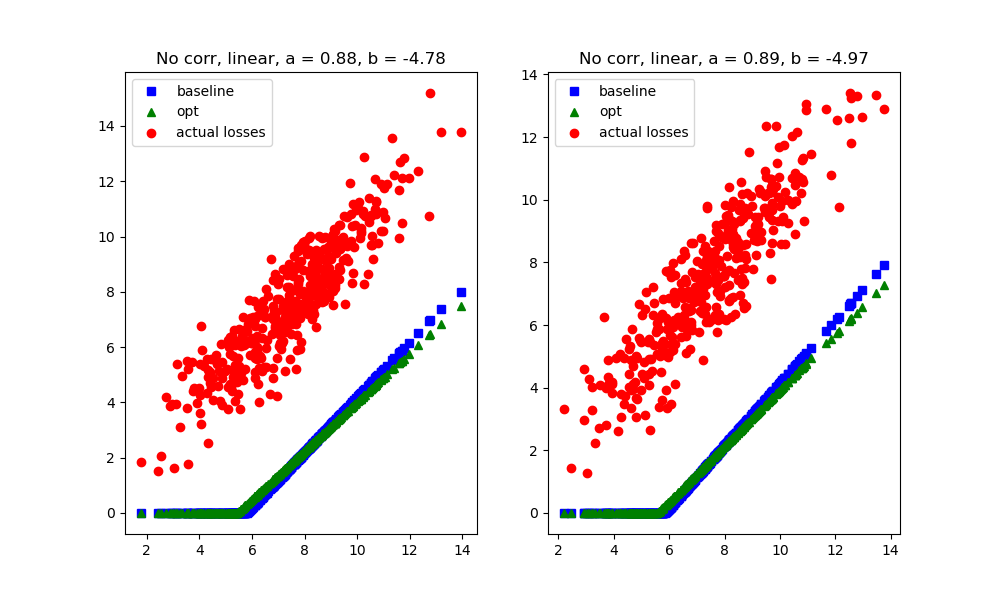
\includegraphics[width=0.75\textwidth]{../../output/figures/Exploration/no_correlation_linear.png}
    \end{figure}

    \begin{table}[H]
        \centering
        \small
        \caption{Performance Metrics}
        \resizebox*{\columnwidth}{!}{\begin{tabular}{lrrrr}
\toprule
{} &  $|L_2 - L_1|$ &  $P(L > Q(0.6))$ &  Required Capital &  TotalCost \\
\midrule
Baseline &       0.04 &             0.02 &              7.33 &    1529.13 \\
Opt      &       0.01 &             0.02 &              6.61 &    1537.30 \\
\bottomrule
\end{tabular}
}
    \end{table}


    \subsubsection{Positive Correlation Case}
    \begin{figure}[H]
        \centering
        \caption{Positive Correlation, model correctly specified}
        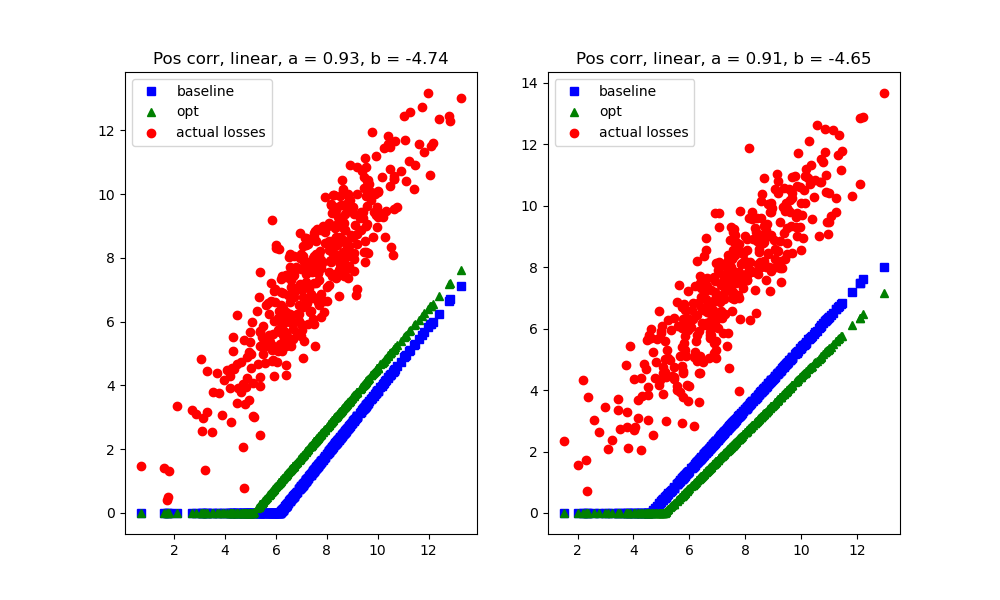
\includegraphics[width=0.75\textwidth]{../../output/figures/Exploration/pos_correlation_linear.png}
    \end{figure}

    \begin{table}[H]
        \centering
        \small
        \caption{Performance Metrics}
        \resizebox*{\columnwidth}{!}{\begin{tabular}{lrrrr}
\toprule
{} &  $|L_2 - L_1|$ &  $P(L > Q(0.6))$ &  Required Capital &  TotalCost \\
\midrule
Baseline &       1.26 &             0.02 &              9.08 &    1798.04 \\
Opt      &       0.10 &             0.01 &              8.48 &    1814.20 \\
\bottomrule
\end{tabular}
}
    \end{table}

    \subsubsection{Negative Correlation Case}
    \begin{figure}[H]
        \centering
        \caption{Negative Correlation, model correctly specified}
        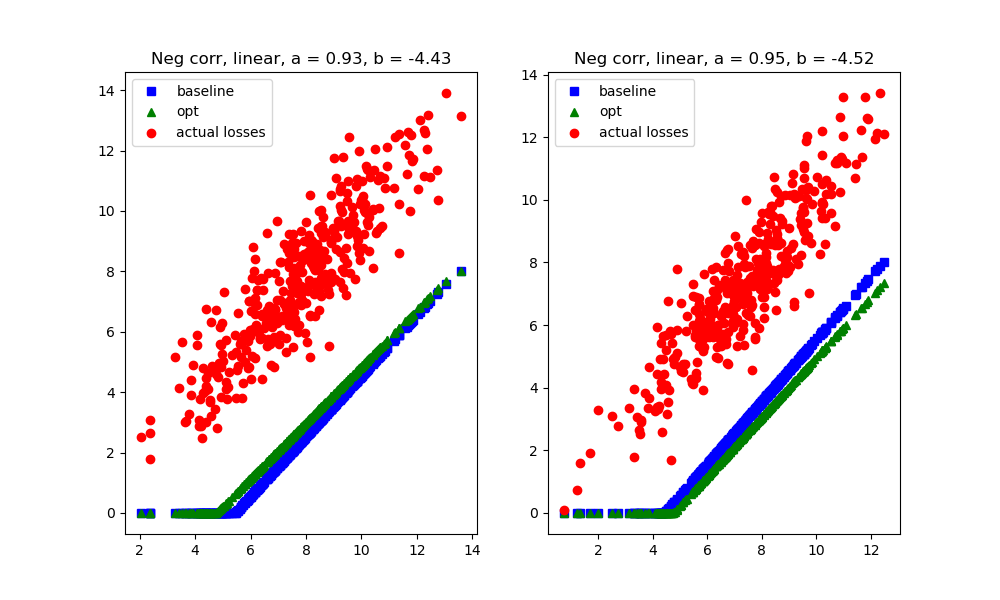
\includegraphics[width=0.75\textwidth]{../../output/figures/Exploration/neg_correlation_linear.png}
    \end{figure}

    \begin{table}[H]
        \centering
        \small
        \caption{Performance Metrics}
        \resizebox*{\columnwidth}{!}{\begin{tabular}{lrrrr}
\toprule
{} &  $|L_2 - L_1|$ &  $P(L > Q(0.6))$ &  Required Capital &  TotalCost \\
\midrule
Baseline &       0.89 &             0.00 &              3.18 &    2164.09 \\
Opt      &       0.08 &             0.00 &              3.04 &    2154.15 \\
\bottomrule
\end{tabular}
}
    \end{table}

    \subsubsection{Disparate Variance Case}
    \begin{figure}[H]
        \centering
        \caption{Unequal Variance, model correctly specified}
        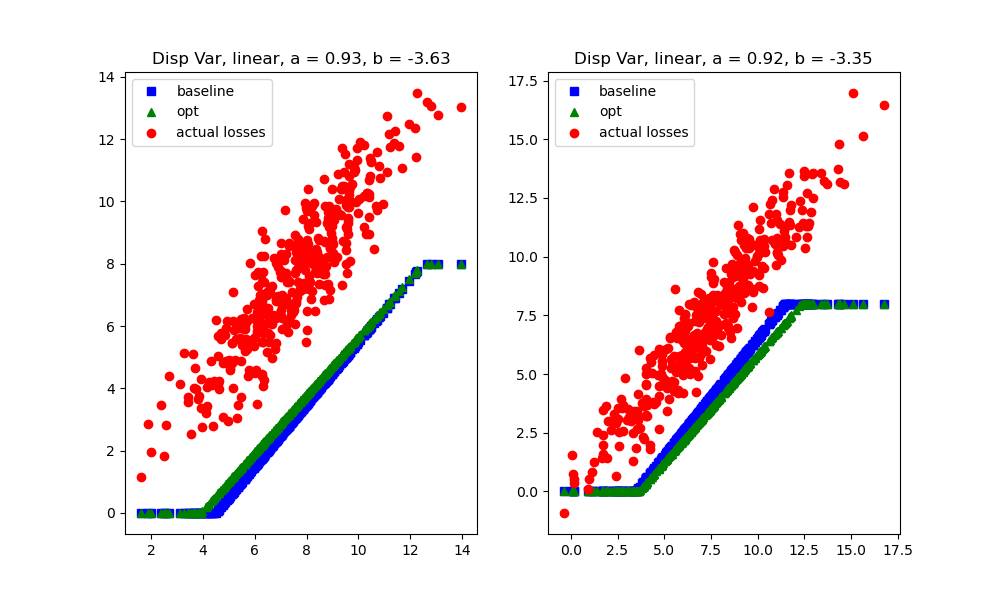
\includegraphics[width=0.75\textwidth]{../../output/figures/Exploration/disp_var_linear.png}
    \end{figure}

    \begin{table}[H]
        \centering
        \small
        \caption{Performance Metrics}
        \resizebox*{\columnwidth}{!}{\begin{tabular}{lrrrr}
\toprule
{} &  $|L_2 - L_1|$ &  $P(L > Q(0.6))$ &  Required Capital &  TotalCost \\
\midrule
Baseline &       1.06 &             0.01 &              7.35 &    2777.54 \\
Opt      &       0.35 &             0.01 &              7.11 &    2746.15 \\
\bottomrule
\end{tabular}
}
    \end{table}

  \subsection{Misspecified Prediction Model}
    \subsubsection{No correlation Case}
    \begin{figure}[H]
        \centering
        \caption{No Correlation, model misspecified}
        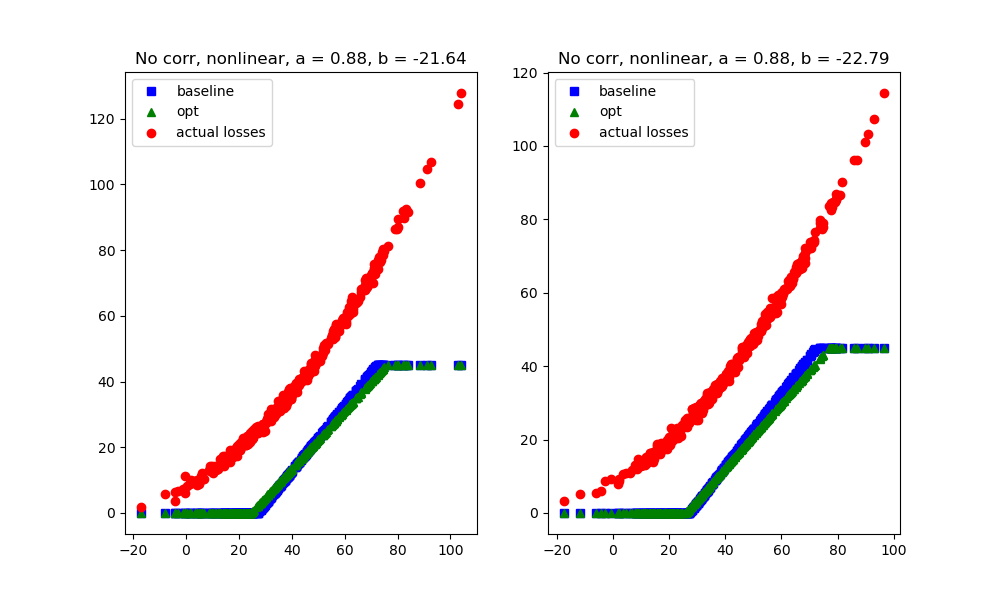
\includegraphics[width=0.75\textwidth]{../../output/figures/Exploration/no_correlation_nonlinear.png}
    \end{figure}

    \begin{table}[H]
        \centering
        \small
        \caption{Performance Metrics}
        \resizebox*{\columnwidth}{!}{\begin{tabular}{lrrrr}
\toprule
{} &  $|L_2 - L_1|$ &  $P(L > Q(0.6))$ &  Required Capital &  TotalCost \\
\midrule
Baseline &           0.39 &             0.06 &             55.53 &   12627.09 \\
Opt      &           1.11 &             0.06 &             52.43 &   12305.87 \\
\bottomrule
\end{tabular}
}
    \end{table}

    \subsubsection{Positive Correlation Case}
    \begin{figure}[H]
        \centering
        \caption{Positive Correlation, model misspecified}
        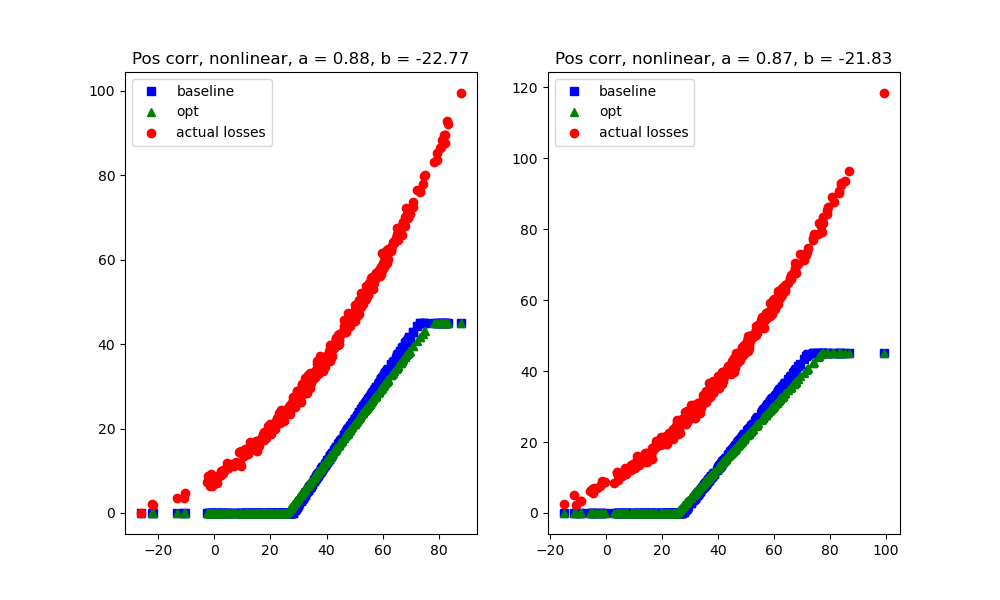
\includegraphics[width=0.75\textwidth]{../../output/figures/Exploration/pos_correlation_nonlinear.png}
    \end{figure}

    \begin{table}[H]
        \centering
        \small
        \caption{Performance Metrics}
        \resizebox*{\columnwidth}{!}{\begin{tabular}{lrrrr}
\toprule
{} &  $|L_2 - L_1|$ &  $P(L > Q(0.6))$ &  Required Capital &  TotalCost \\
\midrule
Baseline &           0.14 &             0.03 &             59.46 &   12220.84 \\
Opt      &           0.16 &             0.03 &             60.27 &   11896.31 \\
\bottomrule
\end{tabular}
}
    \end{table}

    \subsubsection{Negative Correlation Case}
    \begin{figure}[H]
        \centering
        \caption{Negative Correlation, model misspecified}
        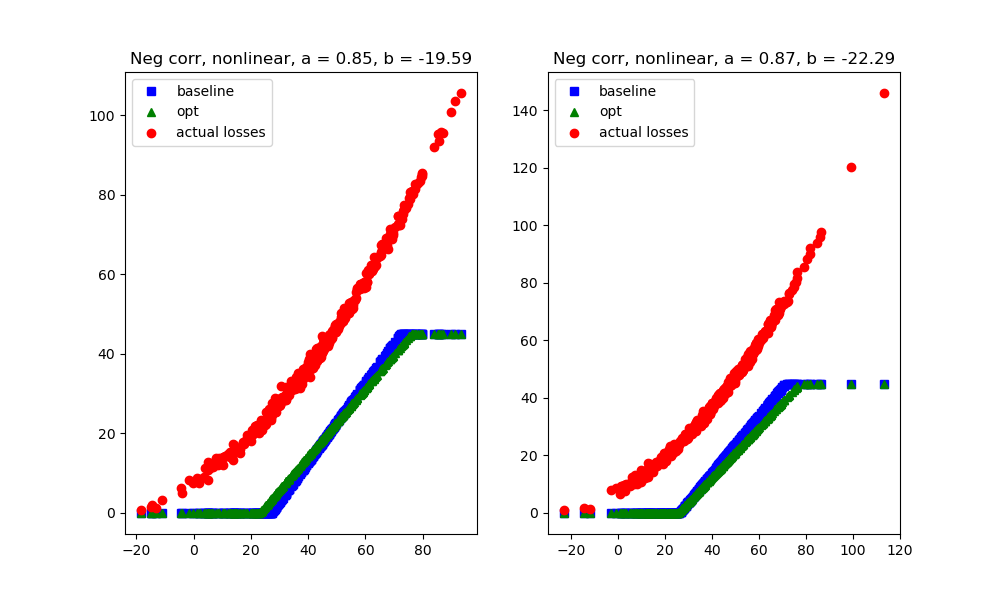
\includegraphics[width=0.75\textwidth]{../../output/figures/Exploration/neg_correlation_nonlinear.png}
    \end{figure}

    \begin{table}[H]
        \centering
        \small
        \caption{Performance Metrics}
        \resizebox*{\columnwidth}{!}{\begin{tabular}{lrrrr}
\toprule
{} &  $|L_2 - L_1|$ &  $P(L > Q(0.6))$ &  Required Capital &  TotalCost \\
\midrule
Baseline &           0.97 &             0.04 &             28.99 &   13690.87 \\
Opt      &           1.07 &             0.04 &             26.75 &   13248.34 \\
\bottomrule
\end{tabular}
}
    \end{table}

    \subsubsection{Disparate Variance Case}
    \begin{figure}[H]
        \centering
        \caption{Unequal Variance, model misspecified}
        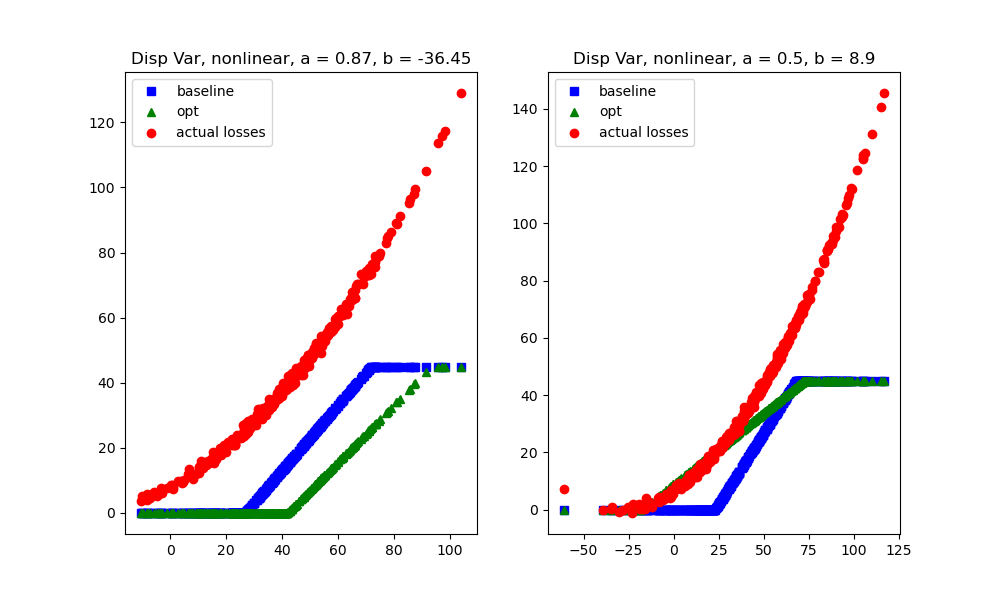
\includegraphics[width=0.75\textwidth]{../../output/figures/Exploration/disp_var_nonlinear.png}
    \end{figure}

    \begin{table}[H]
        \centering
        \small
        \caption{Performance Metrics}
        \resizebox*{\columnwidth}{!}{\begin{tabular}{lrrrr}
\toprule
{} &  $|L_2 - L_1|$ &  $P(L > Q(0.6))$ &  Required Capital &  TotalCost \\
\midrule
Baseline &           4.09 &             0.11 &             53.29 &   14687.41 \\
Opt      &          21.77 &             0.29 &             49.24 &   14101.33 \\
\bottomrule
\end{tabular}
}
    \end{table}

  



\end{document}